\section{Præsentation af data}
\label{TestAfSkalaPraesentationAfData}
%
\begin{figure}[H]
\centering
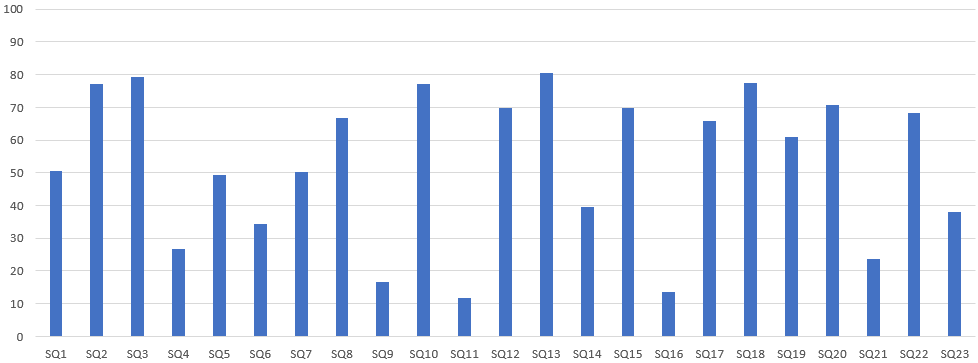
\includegraphics[width = \textwidth]{Figure/DatabehandlingSkalaer/BarPlotRaaData} 
\caption{Barplot over den gennemsnitlige besvarelse til hver skala}
\label{fig:BarPlot}
\end{figure}
\noindent
%
\begin{figure}[H]
\centering
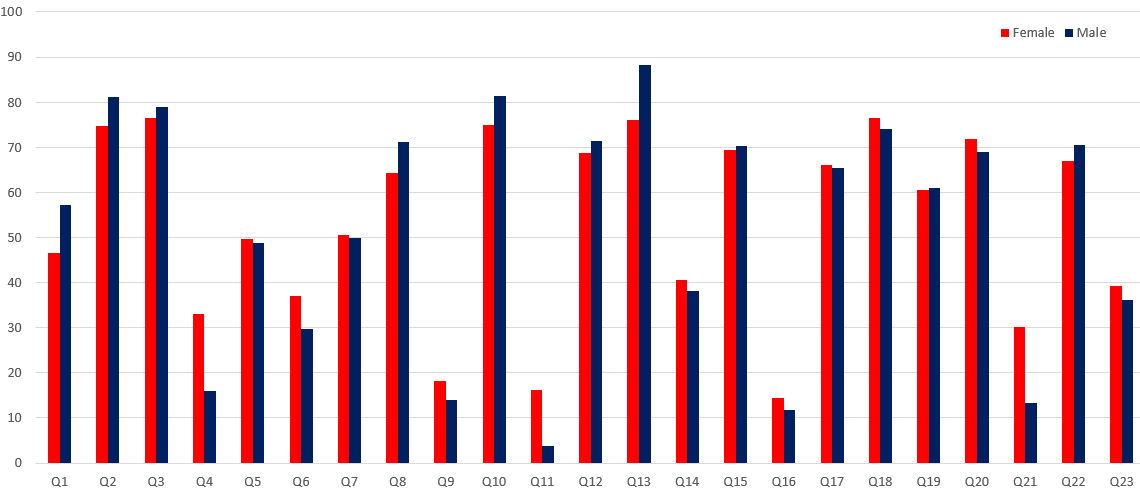
\includegraphics[width = \textwidth]{Figure/DatabehandlingSkalaer/KoenGennemnitligBesvarelser} 
\caption{Barplot over den gennemsnitlige besvarelse til hver skala for mænd og kvinder}
\label{fig:BarPlotKoen}
\end{figure}
\noindent
%
\begin{figure}[H]
\centering
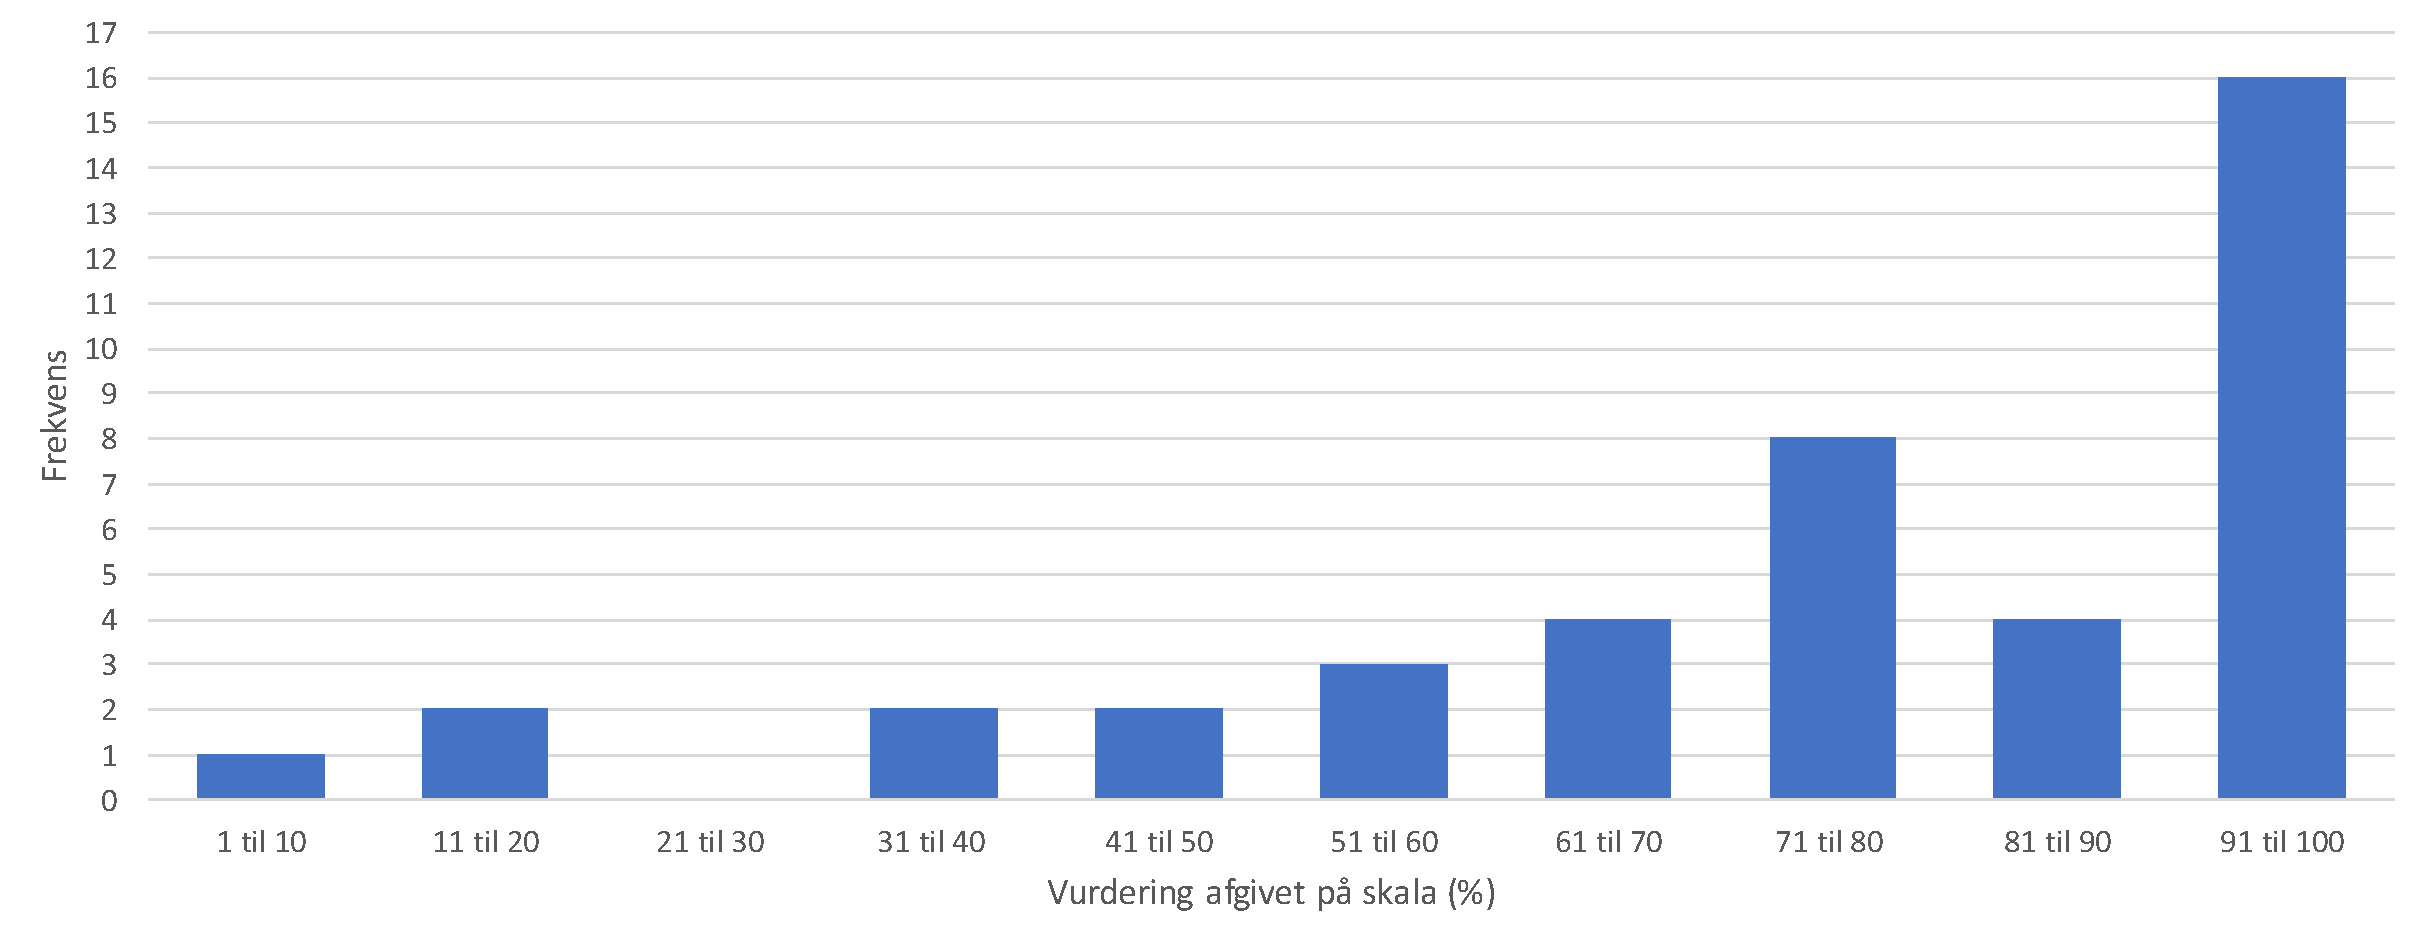
\includegraphics[width = \textwidth]{Figure/DatabehandlingSkalaer/TechFrekvens} 
\caption{Histogram over besvarelserne til spørgsmålet ``Hvor glad er du for teknologi?''}
\label{fig:BarPlotTechFrekvens}
\end{figure}
\noindent
%
\begin{figure}[H]
\centering
\begin{minipage}{.5\textwidth}
  \centering
  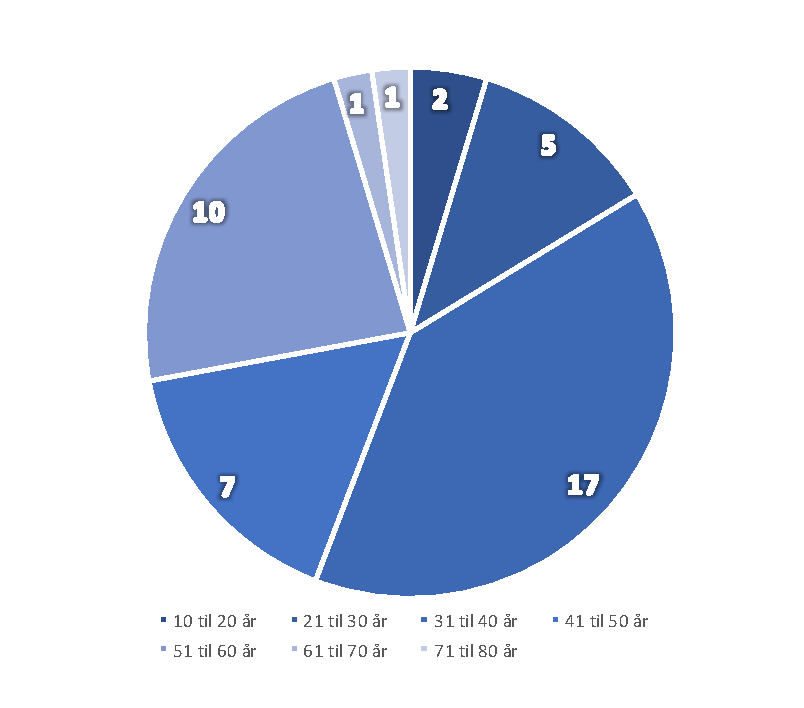
\includegraphics[width=\linewidth]{Figure/DatabehandlingSkalaer/CirkelDiagramAlder}
  \caption{Fordelingen af testpersonernes alder.}
  \label{fig:CirkelDiagramCirkelDiagramAlder}
\end{minipage}%
\begin{minipage}{.5\textwidth}
  \centering
  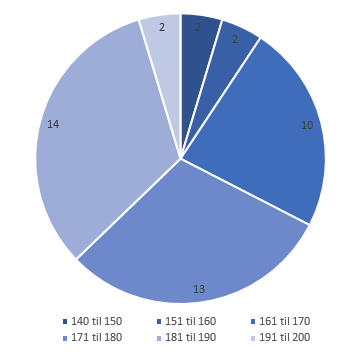
\includegraphics[width=\linewidth]{Figure/DatabehandlingSkalaer/CirkelDiagramHoejde}
  \caption{Fordelingen af testpersonernes højde.}
  \label{fig:CirkelDiagramHoejde}
\end{minipage}
\end{figure}
\noindent
%